%----------------------------------------------------------------------------------------
%	PACKAGES AND THEMES
%----------------------------------------------------------------------------------------
\documentclass[aspectratio=169,xcolor=dvipsnames]{beamer}
\usetheme{Simple}

\usepackage{hyperref}
\usepackage{graphicx} % Allows including images
\usepackage{booktabs} % Allows the use of \toprule, \midrule and \bottomrule in tables
\usepackage{amsmath}  % For math environments like align
\newcommand{\littlebreak}{\vspace{0.2cm}}
%----------------------------------------------------------------------------------------
%	TITLE PAGE
%----------------------------------------------------------------------------------------

% The title
\title[short title]{Lab-Meeting notes: Non-smooth Control Barrier Functions for Safety Critical Systems}
\subtitle{For Safe AI Lab}

\author{Chirayu Salgarkar}
\institute[Mercer] % Your institution may be shorthand to save space
{
    Safe AI Lab, RIT \\

    \vskip 3pt
}
\date{\today} % Date, can be changed to a custom date

%----------------------------------------------------------------------------------------
%	PRESENTATION SLIDES
%----------------------------------------------------------------------------------------

\begin{document}

\begin{frame}
    \titlepage
\end{frame}

\begin{frame}{Overview}
    \tableofcontents
\end{frame}

%------------------------------------------------
\section{Control Theory Fundamentals}
%------------------------------------------------

\begin{frame}{Motive of Controller Synthesis}
\textbf{Goal:} Design a controller, or a combination of components, so that any system has some desired characteristics.
\bigbreak
  Such desired outputs are:
  \setbeamertemplate{itemize items}[triangle]
  \begin{itemize}
  \item Stability
  \item Following command signals, or tracking
  \item Reduce the response to external disturbances
  \end{itemize}  
\end{frame}
   
\begin{frame}{Background}  
  \setbeamertemplate{itemize items}[triangle]
  \begin{itemize}
    \item A control system, in its simplest form, is just a combination of components that act together to perform a desired objective. \textbf{(input $\to$ output)}
   \item In classical control, most problems and situations are treated as a single-input single-output (SISO) system. That does not allow us to see anything with respect to the interior structure of the system. 
    \item Modern control theory handles this by describing plant dynamics as a set of coupled first-order ODEs in a set of \textit{state variables}. Think of state variables as internal variables. We then use a set of algebraic equations to combine state variables into physical output variables. 
  \end{itemize}
\end{frame}

%------------------------------------------------

\begin{frame}{Background}
    The set of \textbf{internal} variables necessary to describe a system and its response to any inputs is known as the  \alert{state}. Knowing the state allows us to generate a \alert{state-determined system} model. 
    \bigbreak
    \begin{block}{State-determined Systems}
        A \textit{state-determined system} has the characteristic that given the mathematical description of the system, as well as the initial time conditions of such variables, and system inputs for time $t > t_0$, we can predict future system state and outputs for all $t > t_0$. 
    \end{block}
\end{frame}

%------------------------------------------------

\begin{frame}{Cyber-physical systems and Safety-Critical Control}
    \setbeamertemplate{itemize items}[triangle]
    \begin{itemize}
    \item \textit{Cyber-physical systems} integrate sensing, computation, control, and networking into physical objects and infrastructure (NSF).
    \end{itemize} 
    
    \underline{Individual controller synthesis is not easy in large-scale systems.}
    Why?
    \begin{itemize}
    \item Messy integration
    \item Different desired outputs for each component (safety + performance)
    \item Difficulty enforcing parameters for safety-critical control
    \end{itemize} 
    Any engineered system should be designed as safe! (Eg. ACC)
    \bigbreak
    \textbf{New Goal:} Design a controller, or a combination of components, so that any system has some desired characteristics, but \textit{always maintains safety-critical properties}.
\end{frame}
\section{Rendering systems invariant}
\begin{frame}{Rendering a system invariant}
        \textbf{Methods}
        \begin{enumerate}
            \item \color{ForestGreen}{Lyapunov Theory}
            \color{RawSienna}
            \item Nagumo's Invariance Principle
            \item \color{ForestGreen}{Control Lyapunov Function}
            \color{RawSienna}
            \item Control Barrier Function
        \end{enumerate}
\end{frame}

%------------------------------------------------

\begin{frame}{Lyapunov Theory}
    \begin{theorem}[Lyapunov Theory]
        Given a dynamical system $\dot{x} = f(x)$, for a function $f: \mathbb R ^n \to \mathbb R ^n$, if you can devise a function $V: \mathbb R ^n \to \mathbb R$ such that 
        \begin{enumerate}
        \item $V(x_e) = 0, V(x) > 0$ if $x \neq x_e$
        \littlebreak
        \item $\dot{V}(x) = \nabla V(x) f(x) < 0$ if $x \neq x_e$
        \end{enumerate}
        Your system maintains the stability property. 
    \end{theorem}
\end{frame}

%------------------------------------------------

\begin{frame}{Sketch}
    \begin{figure}
    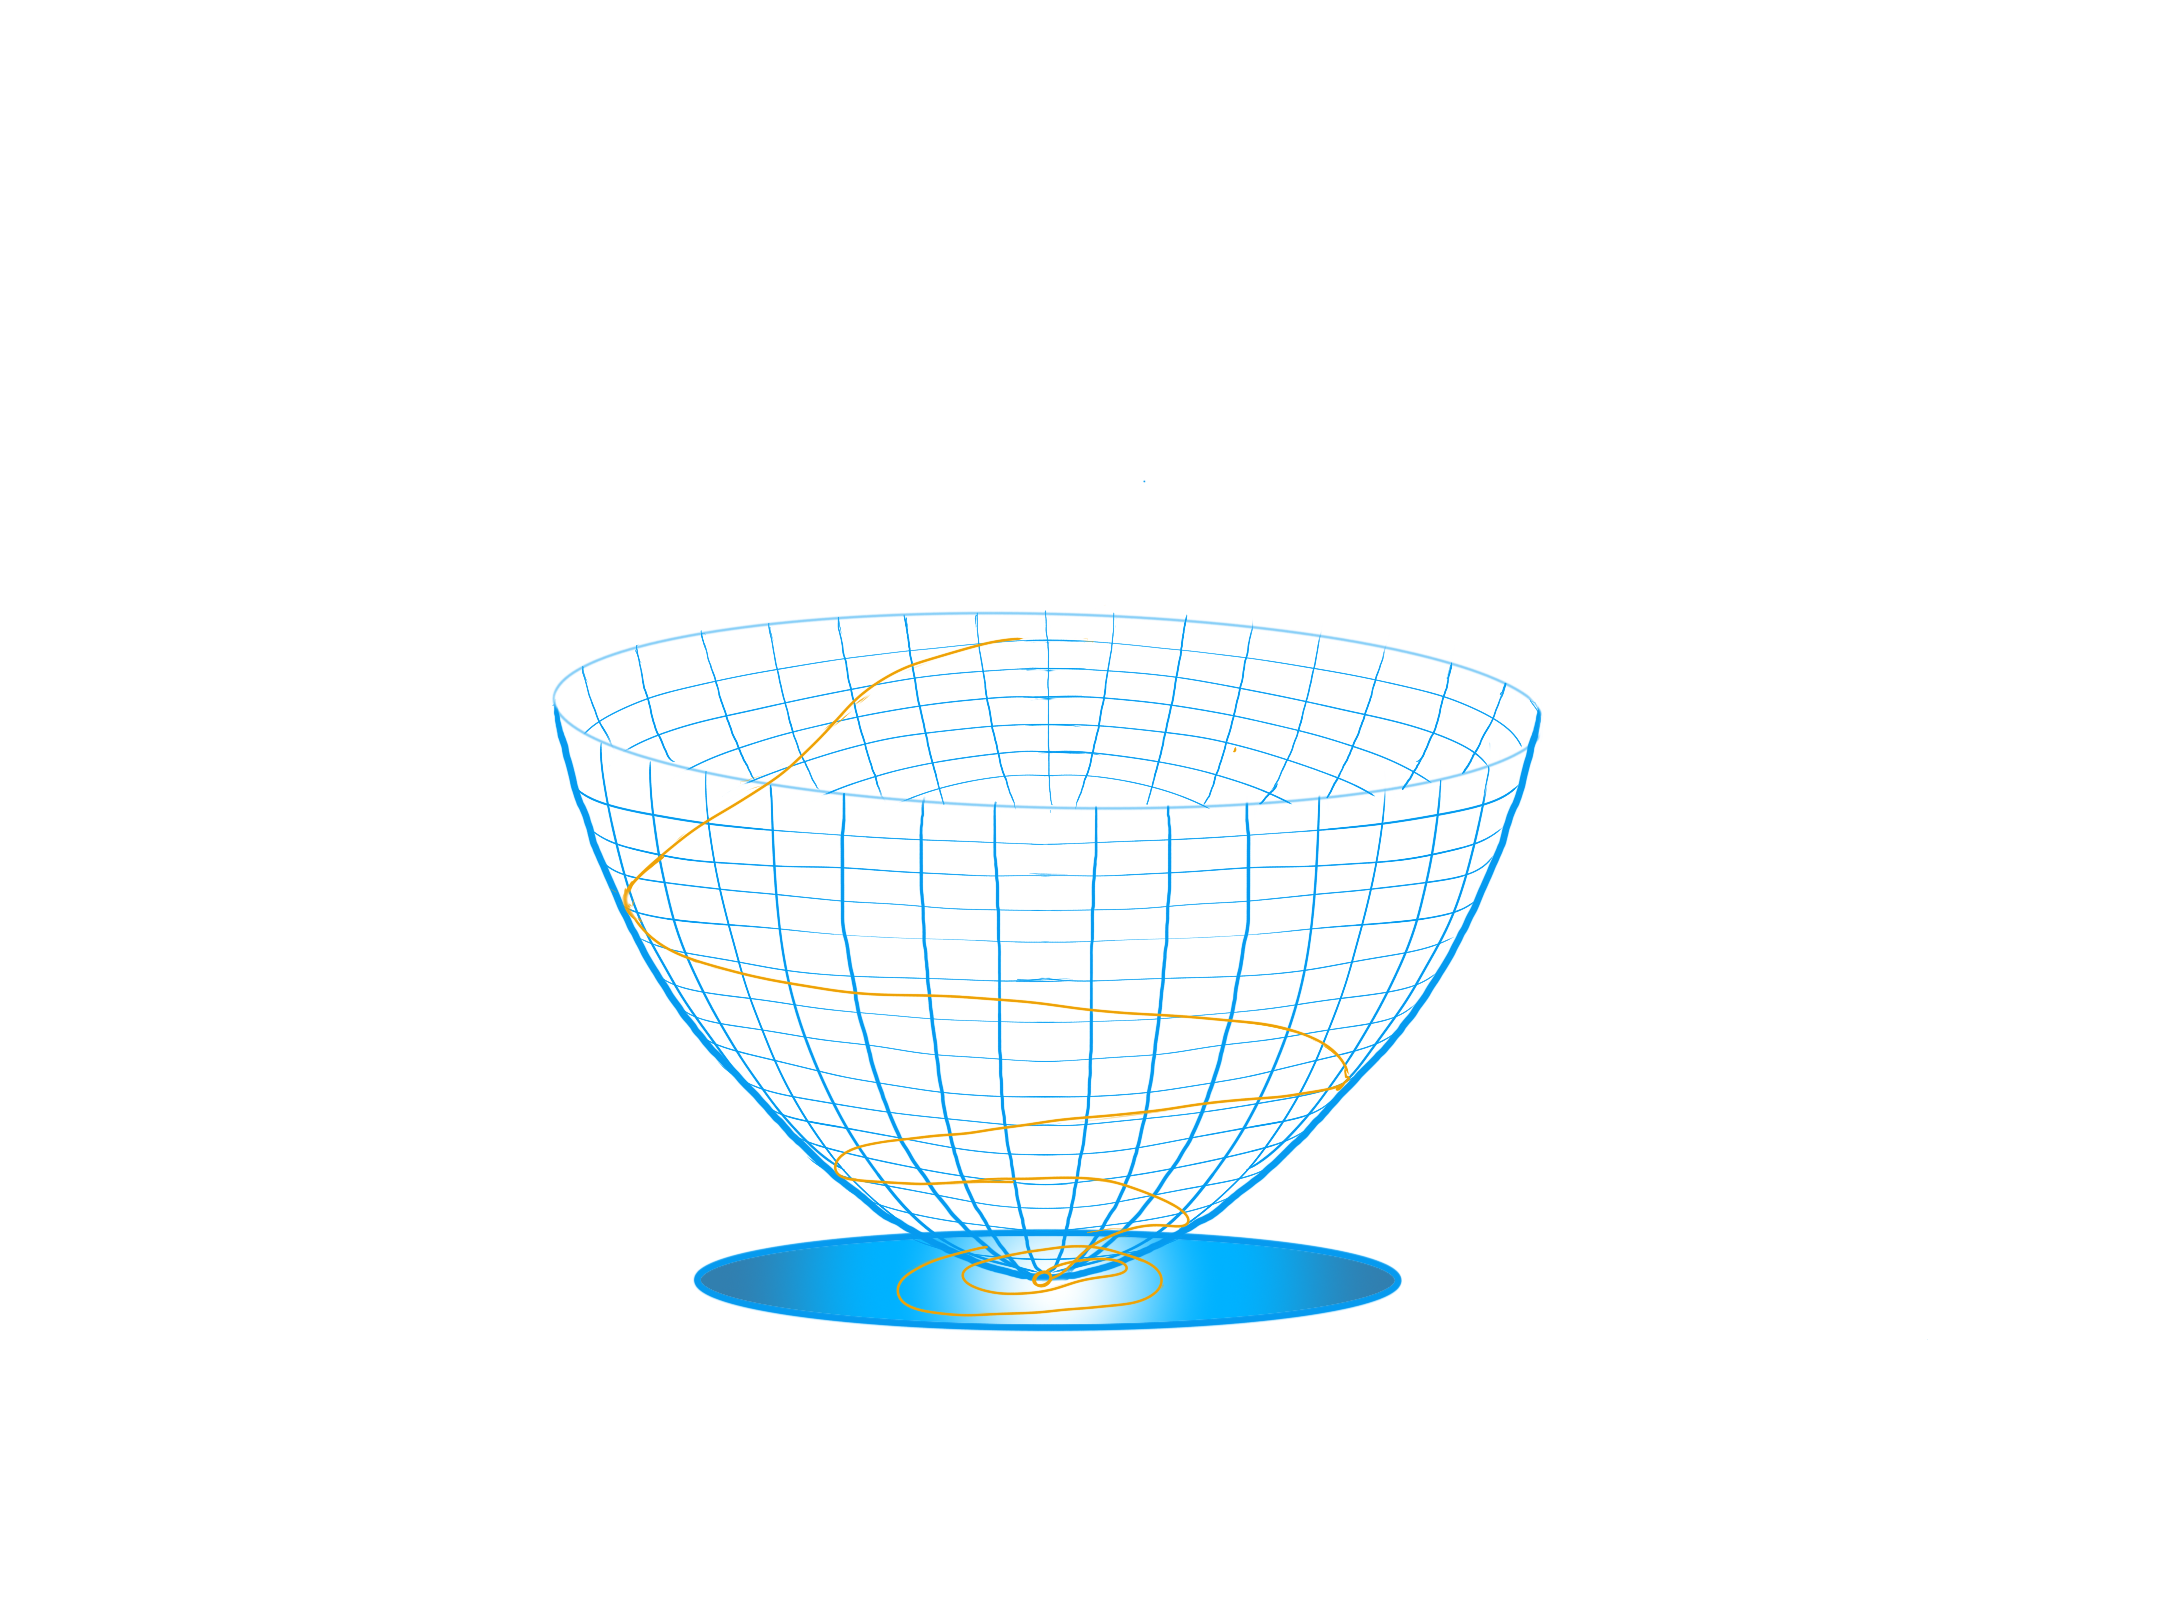
\includegraphics[width=0.5\linewidth]{Untitled 64.png}
    \end{figure}
    Note that the function is imbued onto the original sketch of the system below.
\end{frame}

%------------------------------------------------

\begin{frame}{Nagumo's Invariance Principle}
    \begin{theorem}[]
        Given a dynamical system $\dot{x} = f(x)$ for a function $f: \mathbb R ^n \to \mathbb R ^n$ and a desired safe set $\mathcal C \subseteq \mathbb R ^n$, if you can produce a smooth function $h: \mathbb R ^n \to \mathbb R$ such that $\mathcal C = \{x \in \mathbb R ^n \; | \; h(x) \geq 0 \}$ and $\nabla h(x) \neq 0$ whenever $h(x) = 0$, then the system is forward-invariant on $\mathcal C$ if and only if $\dot{h} (x) \geq 0$ for each $x \in \partial \mathcal C = \{x \in \mathbb R ^n \; | \; h(x) = 0 \}$.
    \end{theorem}
\end{frame}

%------------------------------------------------


\begin{frame}{Control Barrier Function   }
Consider the case of a control affine system, a specific nonlinear system, such that:
$\dot{x} = f(x) + g(x)u$, where $f: \mathbb R^n \to \mathbb R^n$ is the autonomous system dynamics, $u$ represents the control input and $g: \mathbb R^n \to \mathbb R^n$ is the actuating term of such an input.

Note: This is analogous to most interpretations of dynamical systems.

Now, we have a new goal: we seek to look for control invariance, rather than simply forward invariance.



    \begin{theorem}[Control Lyapunov Function]
        Given a control system $\dot{x} = f(x) + g(x)u$, if you can devise a function $V:\mathbb R^n \to \mathbb R$ such that: 
                \begin{enumerate}
        \item $V(x_e) = 0, V(x) > 0$ if $x \neq x_e$, and
        \littlebreak
        \item There exists a control input $u: \mathbb R^m \to \mathbb R^n$ such that $\dot{V}(x, u) < 0$ if $x \neq x_e$,
        \end{enumerate}
        then with that control input, the system will converge to the equilibrium point $x_e$.
    \end{theorem}
\end{frame}

\begin{frame}{Control Barrier Function}
Now, apply the control affine definition to Nagumo's Invariance Principle, and we get the definition of a CBF.

    \begin{theorem}[Control Barrier Function ]
    {\bf [Ames, Coogan, Egerstedt et al, 2019].}
        Given a control system $\dot{x} = f(x) + g(x)u$, if you can devise a function $B: \mathbb R^n \to \mathbb R$ such that: 
        \begin{enumerate}
        \item B(x) is continuously differentiable with nonzero gradient at the boundary, and
        \item There exists a strictly increasing function $\gamma$ such that:
        \begin{itemize}
            \item [a.] $\gamma (0) = 0$, and
            \item [b.] The supremum of $\nabla{V(x)}f(x)+\nabla{V(x)}g(x)u + \gamma (B(x))$, taken with respect to the control variable $u$, is greater than or equal to $0$ for all $x \in \mathcal C$,
        \end{itemize} 
        \end{enumerate}
        then there exists a valid control input such that the system will stay in the safe set.
    \end{theorem}
\end{frame}

\begin{frame}{Why Control Barrier Functions?}
This above function provides a formal safety guarantee that a particular control-affine system is within the safe set. This is especially useful for dynamical systems where safety, or more specifically, invariance, is necessary, such as adaptive cruise control. 
\bigbreak
\textbf{However:}
\end{frame}


\begin{frame}{Drawback}
The specific definition is very conservative. 
This CBF definition only accounts for a small subset of valid functions to guarantee safety-critical control. It is very computationally intensive to find all valid functions, but there is incentive to do better. 
\bigbreak
Suppose we relax the condition that B(x) is continuously differentiable with nonzero gradient at the boundary. 
\end{frame}

\begin{frame}{Proposition}
We propose a new requirement: B(x) need not be continuously differentiable, but rather just left limit differentiable. 
\bigbreak
Dr. Makhin Thitsa helped show that this easing of a restriction still guarantees that the members remain within the safe set. 

This is useful, because it is a less conservative definition, allowing for the contruction of functions such as absolute value functions. 
\end{frame}

\begin{frame}{Formal Definition
}
Consider the control affine system 
\begin{equation}
\label{eq:Affine-control-sys}
\dot{x}=F(x)+G(x)u
\end{equation}
and a nonsmooth CBF candidate
$h(x)$. If $r\textsuperscript{th}$ order left derivative $D^r\_h(t)$ exists, and $r$ is the lowest order left derivative where $u$ appears explicitly, then $h$ is said to have {\bf relative degree $r$} with respect to the system in \ref{eq:Affine-control-sys}.
\end{frame}
%%%%%%%%%%%%%%%%%%%%%%%%%%%%%%%%%%%%%%%%%%%%%%%%%%%%%%
% Theorem: Higher Order Comparison Lemma with left derivative condition
%%%%%%%%%%%%%%%%%%%%%%%%%%%%%%%%%%%%%%%%%%%%%%%%%%%%%

\begin{frame}{Formal Definition}
    
\begin{theorem}
\label{th:Higher-order-comparison-lemma-with-left-derivative-condition}
{\bf [Walter, 1970].} If $w(0)\geq 0$ and $D\_w(t)\geq -\beta w(t)$, for $t\in [0,T]$, then, $w(t)\geq 0,\;\forall t\in[0,T]$. Here, $\beta>0$.
\end{theorem}
%%%%%%%%%%%%%%%%%%%%%%%%%%%%%%%%%%%%%%%%%%%
% Definition: Safe set of Higher Order Barrier Function
%%%%%%%%%%%%%%%%%%%%%%%%%%%%%%%%%%%%%%%%%%%%
Let $h$ be $r^\textsuperscript{th}$ order left differentiable and let $h=\psi_0$. Define a sequence of functions such as
%\[
%\psi_k(t)=D\_\psi_{k-1}(t)+\beta_k\psi_{k-1}(t),
%\]
\[
\psi_k(x) = D\_\psi_{k-1}(x)+\beta_k\psi_{k-1}(x),
\]
and a sequence of sets
$C_k=\{\psi_k(x)\geq 0\}$, $1\leq k\leq r$. Define  $C^*=\cap_{k=1}^{r-1}\psi_k(x)$. The function $h$ is {\bf $r\textsuperscript{th}$ order nonsmooth barrier function} %if $\beta_1,\ldots,\beta_r>0$ and a nonempty $C^*$ exist such that
if $\beta_1,\ldots,\beta_r>0$, $C^*$ is nonempty, and there exists a control input $u$ such that $\psi_r(x,u)\geq 0$.
\end{frame}

\begin{frame}{Or more simply,}
    \begin{figure}
    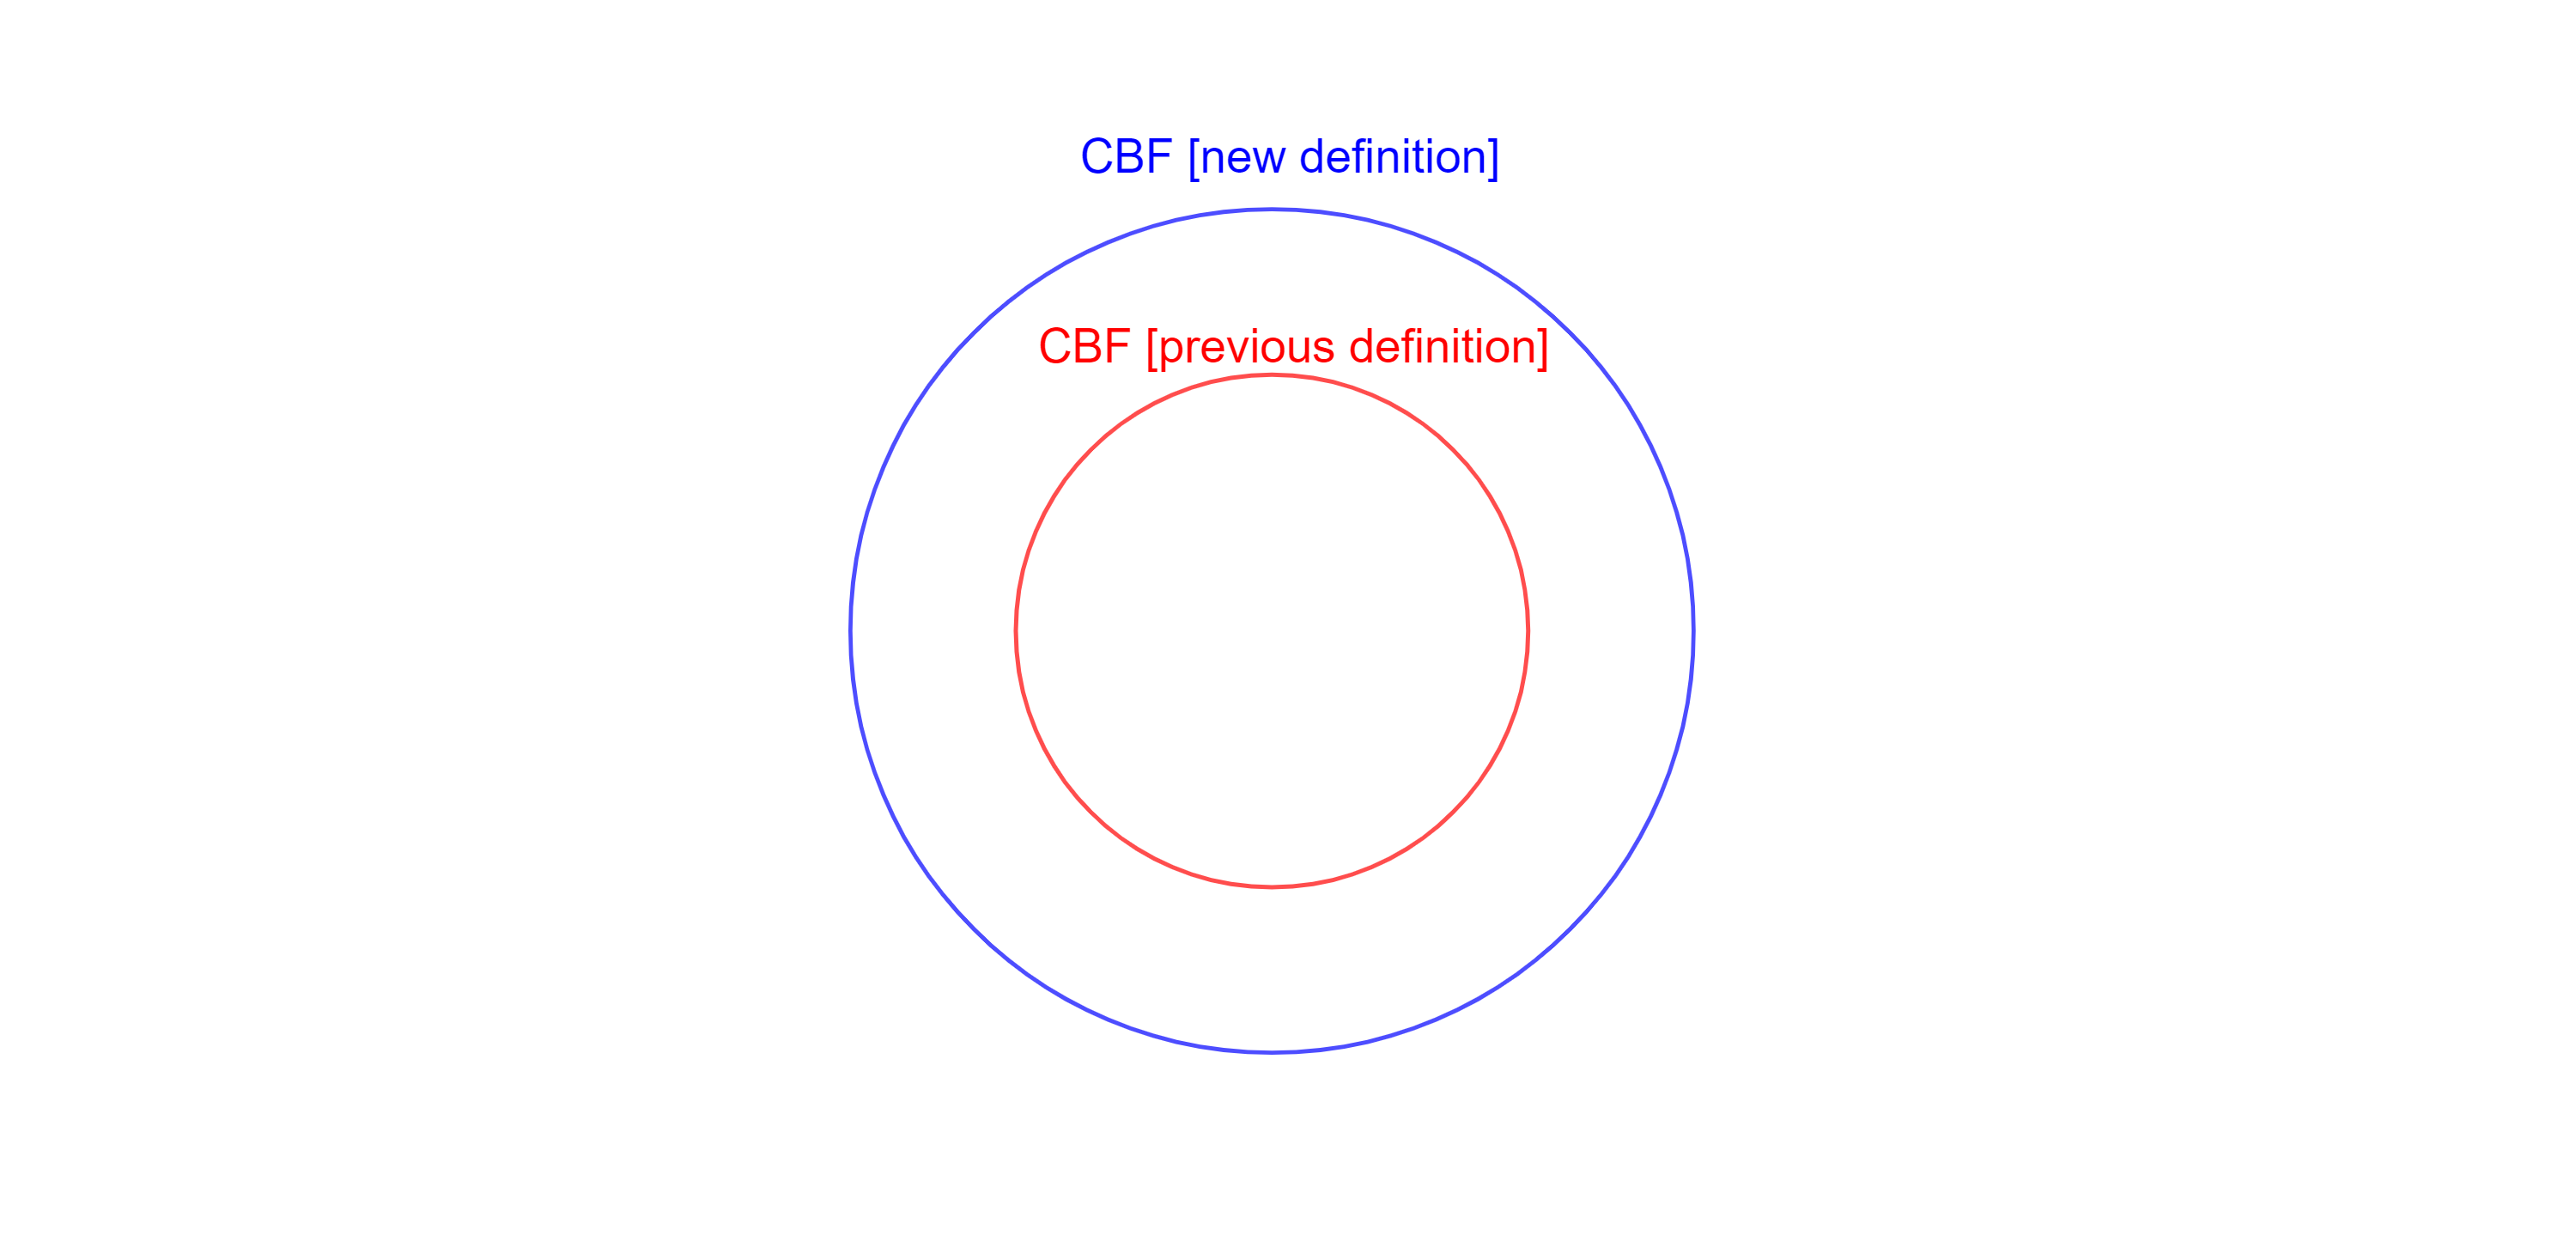
\includegraphics[width=0.8\linewidth]{cbf diagram.png}
    \end{figure}
\end{frame}

\section{Numerical Examples}


\begin{frame}{Numerical Example 1}
    \begin{figure}
    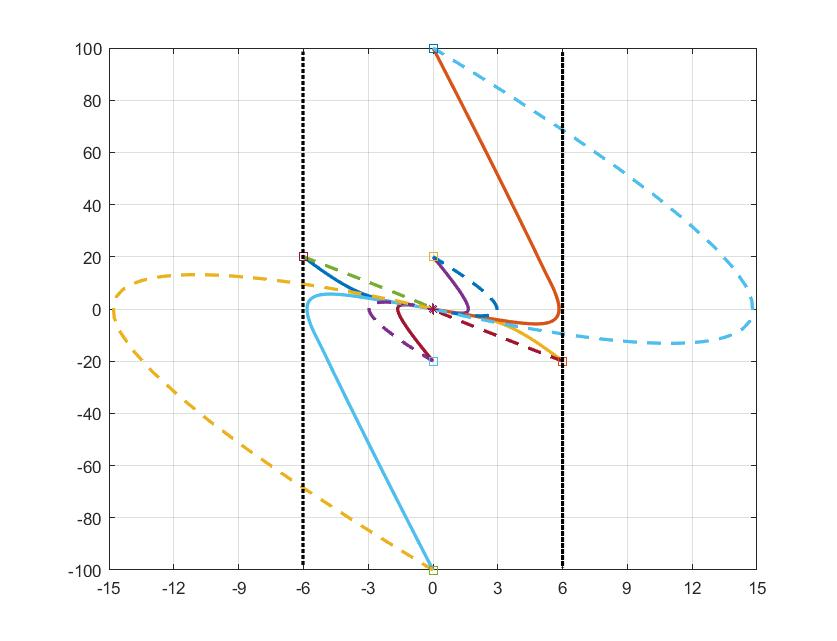
\includegraphics[width=0.4\linewidth]{OutputOfFig1CBFbeta20.jpg}
    \caption{The trajectory obtained using nominal control law (dashed) is seen to go outside $C^*$ with $x_1$ exceeding $6$ for the initial conditions $(0,100)$ and $(0,-100)$. However, when the nonsmooth CBF with $\beta_1=\beta_2=400$ is implemented, the trajectory (solid) is contained in $C^*$.In both cases the states converges to the origin.}
    \end{figure}
\end{frame}


\begin{frame}{Numerical Example 2}
    \begin{figure}
    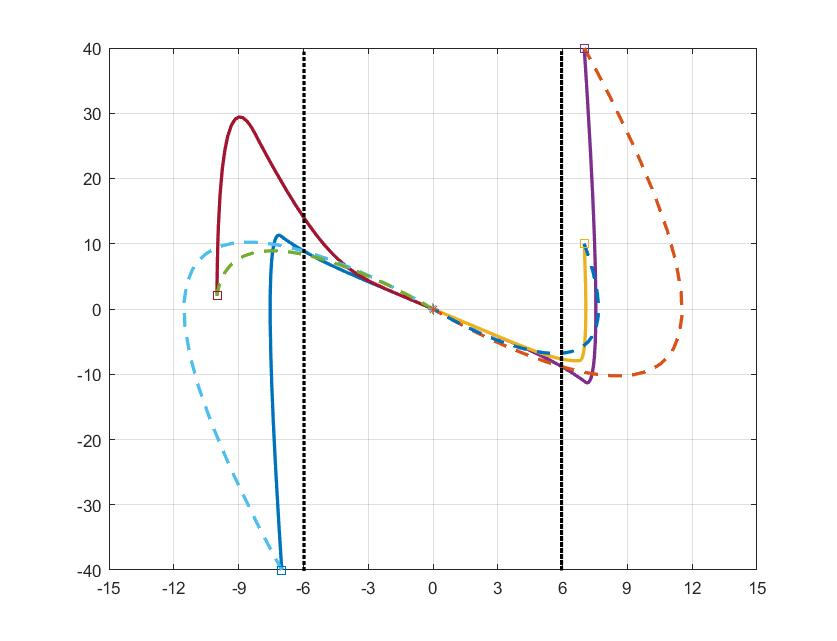
\includegraphics[width=0.4\linewidth]{OutputOfFig2CBFbeta20.jpg}
    \caption{The same initial conditions are used as in previous example. This time the nonsmooth CBF is implemented with $\beta_1=\beta_2=20$. All trajectories produced nonsmooth CBF controller stay within $C^*$. The smaller $\beta_1,\beta_2$ values forces the trajectories to move away from the boundary of $C^*$.}
    \end{figure}
\end{frame}

%------------------------------------------------

\begin{frame}[fragile] % Need to use the fragile option when verbatim is used in the slide
    \frametitle{Summary - Section 1}
    \begin{itemize}
    \item Large-scale engineered systems should be designed as safe.
   \item One way to formally guarantee safety in control systems is through the implementation of a control barrier function. However, this is a very conservative guarantee.
    \item The relaxation of one of the conditions of the CBF, that being continuous differentiability, allows for more control inputs and states to be used, while guaranteeing that such conditions are still safe. 
    \end{itemize}
\end{frame}

% Slide 2: Motivation
\section{Motivation}
\begin{frame}
    \frametitle{Motivation}
    \begin{itemize}
        \item Control systems are often subject to safety constraints, ensuring the system remains within safe operational bounds.
        \item Barrier functions (CBFs) are typically used to enforce these constraints, but most approaches assume smoothness or Lipschitz continuity.
        \item Nonsmooth candidate functions frequently arise, leading to discontinuous control strategies.
    \end{itemize}
\end{frame}

% Slide 3: High-Order Discontinuous CBFs
\section{High-Order Discontinuous CBFs}
\begin{frame}
    \frametitle{Discontinuous High-Order CBFs}
    \begin{itemize}
        \item Traditional CBF approaches assume the smoothness of the function, but real systems may exhibit discontinuities.
        \item We propose methods using piecewise-defined barrier functions that are continuously differentiable within each region but potentially discontinuous at the boundaries.
    \end{itemize}
    \vfill
    \centering
    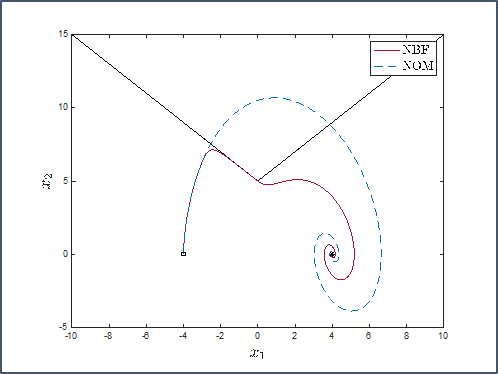
\includegraphics[width=0.4\textwidth]{triple_integrator_system.png}  % Replace with your image path
\end{frame}

% Slide 4: Piecewise-defined Barrier Functions
\section{Piecewise-defined Barrier Functions}
\begin{frame}
    \frametitle{Piecewise-defined Barrier Functions}
    \begin{itemize}
        \item \textbf{Definition:} A piecewise-defined barrier function is one that is continuously differentiable on each segment of an open finite partition.
        \item Each partition has its own local continuously differentiable function ensuring safe behavior within the boundary.
        \item This allows us to enforce safety in systems that have multiple operational modes or discontinuities.
    \end{itemize}
\end{frame}

% Slide 5: Forward Invariance Corollary
\section{Forward Invariance Corollary}
\begin{frame}
    \frametitle{Forward Invariance Corollary}
    \begin{itemize}
        \item Given a system with a piecewise-defined barrier function, if there exists Lipschitz functions on each partition that satisfy certain conditions, then the system is forward invariant.
        \item This means that once the system starts in a safe state, it will remain safe indefinitely, even with discontinuities.
    \end{itemize}
    \vfill
    \centering
\end{frame}

% Slide 6: Simulation Results - Triple Integrator
\section{Simulation Results}
\begin{frame}
    \frametitle{Simulation Results - Triple Integrator System}
    \begin{itemize}
        \item The Triple Integrator system shows how a piecewise-defined barrier function can be used to control a system with discontinuities.
        \item Forward invariance is maintained despite changes in the system’s operational mode.
    \end{itemize}
    \vfill
    \centering
    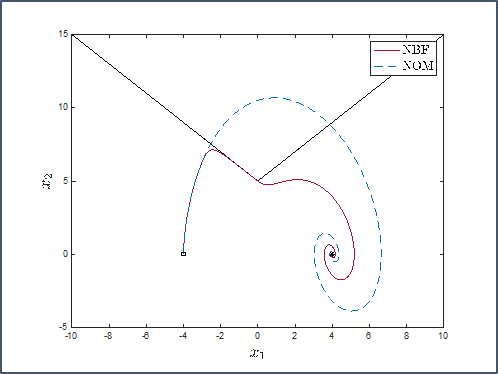
\includegraphics[width=0.4\textwidth]{triple_integrator_system.png}  % Replace with your image path
\end{frame}

% Slide 7: Simulation Results - Second-Order Unicycle
\begin{frame}
    \frametitle{Simulation Results - Second-Order Unicycle System}
    \begin{itemize}
        \item In the second-order unicycle system, we see similar results where the piecewise-defined barrier function ensures forward invariance.
        \item These results demonstrate the general applicability of discontinuous high-order CBFs across different systems.
    \end{itemize}
    \vfill
    \centering
    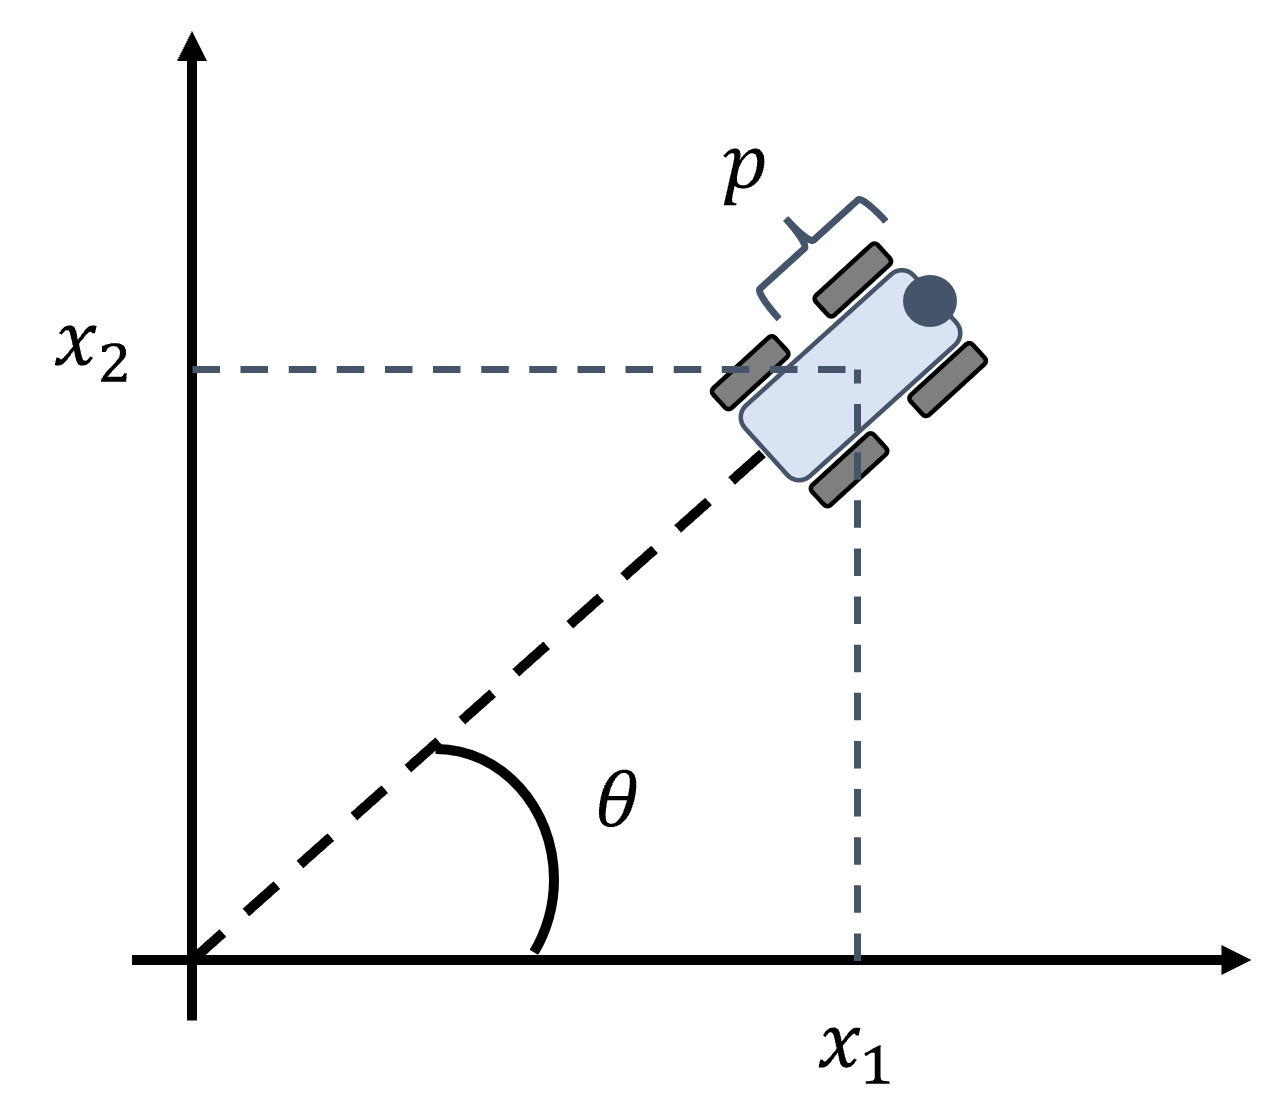
\includegraphics[width=0.4\textwidth]{second_order_unicycle_simulation.png}  % Replace with your image path
\end{frame}

% Slide 8: Conclusion
\section{Conclusion}
\begin{frame}
    \frametitle{Conclusion}
    \begin{itemize}
        \item Discontinuous high-order CBFs provide a powerful framework for controlling systems with nonsmooth dynamics.
        \item Piecewise-defined barrier functions allow for safety guarantees in systems with operational mode changes.
        \item Future work includes exploring extensions to other types of nonsmooth systems and optimizing the computation of these barrier functions.
    \end{itemize}
\end{frame}


\begin{frame}{References}
\begin{enumerate}
    \item A. D. Ames, S. Coogan, M. Egerstedt, et al., {\em Control Barrier Functions: Theory and Applications,} in Proceedings of the 18th European Control Conference (ECC), IEEE, 2019, pp. 3420-3431.
    \item W. Walter, {\em Differential and Integral Inequalities}, Springer, New York City, NY, 1970.
\end{enumerate}
   
\end{frame}


%------------------------------------------------

\begin{frame}
    \Huge{\centerline{The End}}
\end{frame}

%----------------------------------------------------------------------------------------

\end{document}